%\documentclass[10pt]{beamer}
%\usefonttheme[onlylarge]{structurebold}

\documentclass[handout]{beamer}
\usefonttheme[onlylarge]{structurebold}
  \usepackage{pgfpages}
\mode<handout>
\pgfpagesuselayout{4 on 1}[letterpaper,border shrink=5mm]

\hypersetup{
  bookmarks = false,
  colorlinks,
  citecolor = red,
  linkcolor=blue,
  urlcolor=blue,
  pdfpagemode=none,
  pdfstartview={Fit},
  pdftitle={},
  pdfauthor={Michael E. Waugh},
  pdfkeywords={} }
  \setbeamertemplate{navigation symbols}{}

\mode<presentation> {
  \usetheme{boxes}
  % or ...

  \setbeamercovered{transparent}
  % or whatever (possibly just delete it)
}

\setbeamertemplate{itemize subitem}[circle]
\setbeamerfont{frametitle}{size= \large}
\setbeamerfont{ framesubtitle }{size = \footnotesize}
\setbeamertemplate{frametitle}
{
\medskip
\smallskip
{\textsf{\underline{\insertframetitle\phantom{))))))))}}}}}


\usepackage[english]{babel}
\usepackage{wasysym}

\addfootbox{}{\hspace{5cm}\tiny {International Trade---Economics of Global Business, Revised: \today}}%

\title[NYU Stern] % (optional, use only with long paper titles)
{\Large International Trade}

\author[Michael Waugh] % (optional, use only with lots of authors)
{\bf{\Large}}%

\date[] % (optional)

\subject{Talks}

\begin{document}

\begin{frame}
  \titlepage
\end{frame}

%%%%%%%%%%%%%%%%%%%%%%%%%%%%%%%%%%%%%%%%%%%%%%%%%%%%%%%%%%%%%%%%%%%%%%%%%%%%%%%%%%%%%%%%%%%%%%%%%
%%%%%%%%%%%%%%%%%%%%%%%%%%%%%%%%%%%%%%%%%%%%%%%%%%%%%%%%%%%%%%%%%%%%%%%%%%%%%%%%%%%%%%%%%%%%%%%
\begin{frame}[t]
\frametitle{The Plan}
\bigskip
\begin{itemize}
\item Logic of trade
\bigskip
\item Develop Ricardian model of trade. Today\ldots
\begin{itemize}
\medskip
\item Opportunity cost and production possibilities.
\medskip
\item No trade equilibrium.
\medskip
\end{itemize}
\end{itemize}
\end{frame}

%%%%%%%%%%%%%%%%%%%%%%%%%%%%%%%%%%%%%%%%%%%%%%%%%%%%%%%%%%%%%%%%%%%%%%%%%%%%%%%%%%%%%%%%%%%%%%%%
%%%%%%%%%%%%%%%%%%%%%%%%%%%%%%%%%%%%%%%%%%%%%%%%%%%%%%%%%%%%%%%%%%%%%%%%%%%%%%%%%%%%%%%%%%%%%%%%

\begin{frame}[t]
\frametitle{The Logic of Trade}
\bigskip
\begin{itemize}
\item Voluntary exchange is ``win-win''
\begin{itemize}
\medskip
\item Suppose two people or firms value a product or asset differently
\medskip
\item Trade can benefit both
\end{itemize}
\bigskip
\item Example in labor markets:
\begin{itemize}
\medskip
\item You value your time at 50 an hour
\medskip
\item A firm values your time at 60 an hour
\medskip
\item At what price does trade take place?
\medskip
\item Who wins?
\end{itemize}
\end{itemize}
\bigskip
\end{frame}

%%%%%%%%%%%%%%%%%%%%%%%%%%%%%%%%%%%%%%%%%%%%%%%%%%%%%%%%%%%%%%%%%%%%%%%%%%%%%%%%%%%%%%%%%%%%%%%%
%%%%%%%%%%%%%%%%%%%%%%%%%%%%%%%%%%%%%%%%%%%%%%%%%%%%%%%%%%%%%%%%%%%%%%%%%%%%%%%%%%%%%%%%%%%%%%%%

\begin{frame}[t]
\frametitle{The Logic of Trade}
\bigskip
\begin{itemize}
\item Voluntary exchange is ``win-win''
\begin{itemize}
\medskip
\item Suppose two people or firms value a product or asset differently
\medskip
\item Trade can benefit both
\end{itemize}
\bigskip
\item Example in reality:
\begin{itemize}
\medskip
\item Green Bay Packers, Summer 08, 2 good quarterbacks
\medskip
\item NY Jets, none
\medskip
\item Solution:  trade!
\end{itemize}
\end{itemize}
\bigskip
\end{frame}

%%%%%%%%%%%%%%%%%%%%%%%%%%%%%%%%%%%%%%%%%%%%%%%%%%%%%%%%%%%%%%%%%%%%%%%%%%%%%%%%%%%%%%%%%%%%%%%%
%%%%%%%%%%%%%%%%%%%%%%%%%%%%%%%%%%%%%%%%%%%%%%%%%%%%%%%%%%%%%%%%%%%%%%%%%%%%%%%%%%%%%%%%%%%%%%%%

\begin{frame}[t]
\frametitle{The Logic of Trade}
\bigskip
\begin{itemize}
\item Voluntary exchange is ``win-win''
\begin{itemize}
\medskip
\item Suppose two people or firms value a product or asset differently
\medskip
\item Trade can benefit both
\end{itemize}
\bigskip
\item The price often depends on who has the most bargaining power. Consider this game
\begin{itemize}
\medskip
\item We have 100 dollars. Make me an offer on how to split 100 dollars.
\medskip
\item If I agree, we get to keep it. If not 100 dollars is destroyed.
\medskip
\item What offers would money not be destroyed?
\medskip
\item What is the ``Nash equilibrium'' outcome?
\end{itemize}
\end{itemize}
\bigskip
\end{frame}

%%%%%%%%%%%%%%%%%%%%%%%%%%%%%%%%%%%%%%%%%%%%%%%%%%%%%%%%%%%%%%%%%%%%%%%%%%%%%%%%%%%%%%%%%%%%%%%
%%%%%%%%%%%%%%%%%%%%%%%%%%%%%%%%%%%%%%%%%%%%%%%%%%%%%%%%%%%%%%%%%%%%%%%%%%%%%%%%%%%%%%%%%%%%%%%

\begin{frame}[t]
\frametitle{Reasons for International Trade}
\begin{itemize}
\bigskip
\item Relative costs of production, i.e. \textbf{comparative advantage}, rationalize international trade patterns.
\bigskip
\item What shapes a country's comparative advantage\ldots
\begin{itemize}
\bigskip
\item Technology, productivity of workers (absolute advantage).
\bigskip
\item proximity,
\bigskip
\item resources.
\end{itemize}
\end{itemize}
\bigskip
\end{frame}

%%%%%%%%%%%%%%%%%%%%%%%%%%%%%%%%%%%%%%%%%%%%%%%%%%%%%%%%%%%%%%%%%%%%%%%%%%%%%%%%%%%%%%%%%%%%%%%%
%%%%%%%%%%%%%%%%%%%%%%%%%%%%%%%%%%%%%%%%%%%%%%%%%%%%%%%%%%%%%%%%%%%%%%%%%%%%%%%%%%%%%%%%%%%%%%%%

\begin{frame}[t]
\frametitle{Ricardo's Model of Trade}
\bigskip
\begin{itemize}
\item David Ricardo, 1817
\begin{itemize}
\medskip
\item Two goods, countries have fixed productivity at producing them
\medskip
\item In free trade: each country produces one good
\end{itemize}
\bigskip
\item Key concept---comparative advantage
\begin{itemize}
\medskip
\item Each country should produce the good at which it is \begin{alertenv}{comparatively}\end{alertenv} the most productive.
\medskip
\end{itemize}
\end{itemize}
\bigskip
\end{frame}

%%%%%%%%%%%%%%%%%%%%%%%%%%%%%%%%%%%%%%%%%%%%%%%%%%%%%%%%%%%%%%%%%%%%%%%%%%%%%%%%%%%%%%%%%%%%%%%%
%%%%%%%%%%%%%%%%%%%%%%%%%%%%%%%%%%%%%%%%%%%%%%%%%%%%%%%%%%%%%%%%%%%%%%%%%%%%%%%%%%%%%%%%%%%%%%%%

\begin{frame}[t]
\frametitle{Ricardo's Model}
\bigskip
\begin{itemize}
\item Two countries (Home, Foreign), two goods (cloth, wheat), one input (labor)
\bigskip
\item Labor is mobile across sectors.
\bigskip
\item Constant marginal products of labor (MPL):
\end{itemize}
\bigskip
\begin{table}[t]
\begin{center}
\begin{tabular}{lccc}%
\vspace{-0.6cm}\\
\hline%
\hline
\vspace{-.4cm}       &\multicolumn{3}{c}{}\\
                     & Cloth  & Wheat  &  Labor \\%
\vspace{-.4cm}       &\multicolumn{3}{c}{}\\
\hline%
\vspace{-.4cm}       &\multicolumn{3}{c}{}\\
Home                 &   2    &   4     &   25  \\
Foreign              &    1    &    1     &   100  \\
\vspace{-.4cm}       &\multicolumn{3}{c}{}\\
\hline
\end{tabular}
\end{center}
\end{table}
\end{frame}

%%%%%%%%%%%%%%%%%%%%%%%%%%%%%%%%%%%%%%%%%%%%%%%%%%%%%%%%%%%%%%%%%%%%%%%%%%%%%%%%%%%%%%%%%%%%%%%%
%%%%%%%%%%%%%%%%%%%%%%%%%%%%%%%%%%%%%%%%%%%%%%%%%%%%%%%%%%%%%%%%%%%%%%%%%%%%%%%%%%%%%%%%%%%%%%%%


\begin{frame}[t]
\frametitle{Opportunity Cost}
\bigskip
\begin{itemize}
\item Opportunity cost: What you forgo when making a choice
\begin{itemize}
\medskip
\item This context, cloth you give up to make one more unit of wheat
\end{itemize}
\bigskip
\item For the Home
\begin{itemize}
\medskip
\item 1 wheat takes 1/4 units of labor
\medskip
\item 1/4 units of labor could make 1/4$\times2 = 1/2$ cloth
\medskip
\item Opportunity cost of 1 wheat is 1/2 cloth
\end{itemize}
\end{itemize}
\bigskip
\begin{table}[t]
\begin{center}
\begin{tabular}{lccc}%
\vspace{-0.6cm}\\
\hline%
\hline
\vspace{-.4cm}       &\multicolumn{3}{c}{}\\
                     & Cloth  & Wheat  &  Labor \\%
\vspace{-.4cm}       &\multicolumn{3}{c}{}\\
\hline%
\vspace{-.4cm}       &\multicolumn{3}{c}{}\\
Home                 &   2    &   4     &   25  \\
Foreign              &    1    &    1     &   100  \\
\vspace{-.4cm}       &\multicolumn{3}{c}{}\\
\hline
\end{tabular}
\end{center}
\end{table}
\end{frame}

%%%%%%%%%%%%%%%%%%%%%%%%%%%%%%%%%%%%%%%%%%%%%%%%%%%%%%%%%%%%%%%%%%%%%%%%%%%%%%%%%%%%%%%%%%%%%%%
%%%%%%%%%%%%%%%%%%%%%%%%%%%%%%%%%%%%%%%%%%%%%%%%%%%%%%%%%%%%%%%%%%%%%%%%%%%%%%%%%%%%%%%%%%%%%%%

\begin{frame}[t]
\frametitle{PPF and Opportunity Cost}
\vspace{.2cm}
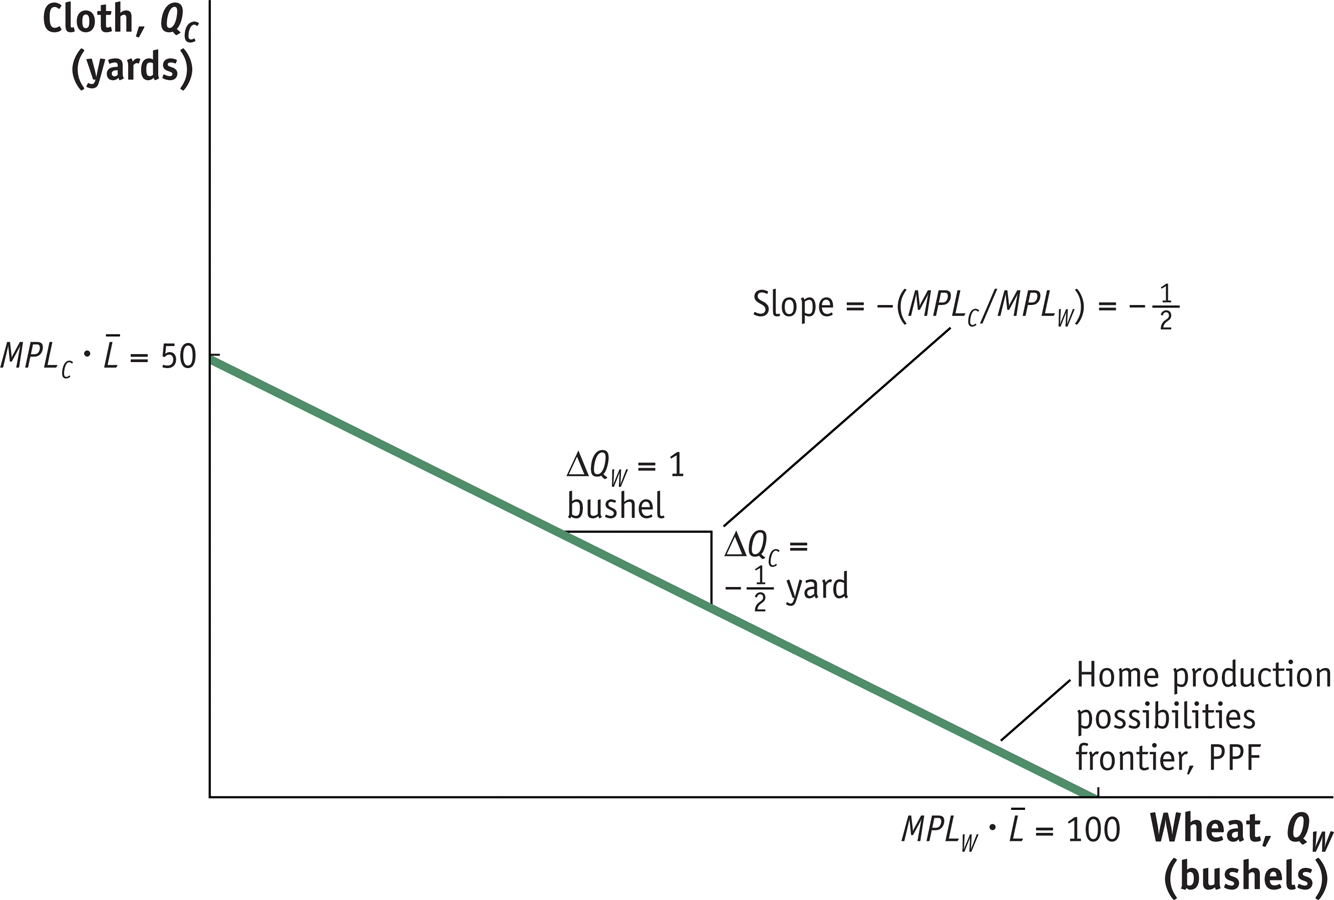
\includegraphics[height=3in,width=4.25in]{Feenstra_Essentials2e_fig_02_01.jpg}
\end{frame}

%%%%%%%%%%%%%%%%%%%%%%%%%%%%%%%%%%%%%%%%%%%%%%%%%%%%%%%%%%%%%%%%%%%%%%%%%%%%%%%%%%%%%%%%%%%%%%%%
%%%%%%%%%%%%%%%%%%%%%%%%%%%%%%%%%%%%%%%%%%%%%%%%%%%%%%%%%%%%%%%%%%%%%%%%%%%%%%%%%%%%%%%%%%%%%%%%


\begin{frame}[t]
\frametitle{Relative Prices}
\begin{itemize}
\item Recall from Chapter 3 Mankiw, profit maximization implies
\begin{eqnarray*}
P \times MPL = W
\end{eqnarray*}
\item In the Ricardian model, workers are free to move and work in the sector paying the highest wages.
\bigskip
\item Thus wages in Cloth sector must equal wages in Wheat sector.
\begin{eqnarray*}
P_w \times MPL_w = W = P_c \times MPL_c\\
\\
\frac{P_w}{P_c} = \frac{MPL_c}{MPL_w} = \frac{2}{4}
\end{eqnarray*}
\medskip
\item The relative price of wheat $=$ the opportunity cost of wheat!
\end{itemize}
\bigskip
\end{frame}

%%%%%%%%%%%%%%%%%%%%%%%%%%%%%%%%%%%%%%%%%%%%%%%%%%%%%%%%%%%%%%%%%%%%%%%%%%%%%%%%%%%%%%%%%%%%%%%%
%%%%%%%%%%%%%%%%%%%%%%%%%%%%%%%%%%%%%%%%%%%%%%%%%%%%%%%%%%%%%%%%%%%%%%%%%%%%%%%%%%%%%%%%%%%%%%%%


\begin{frame}[t]
\frametitle{Equilibrium: Marginal Cost = Marginal Benefit}
\vspace{.2cm}
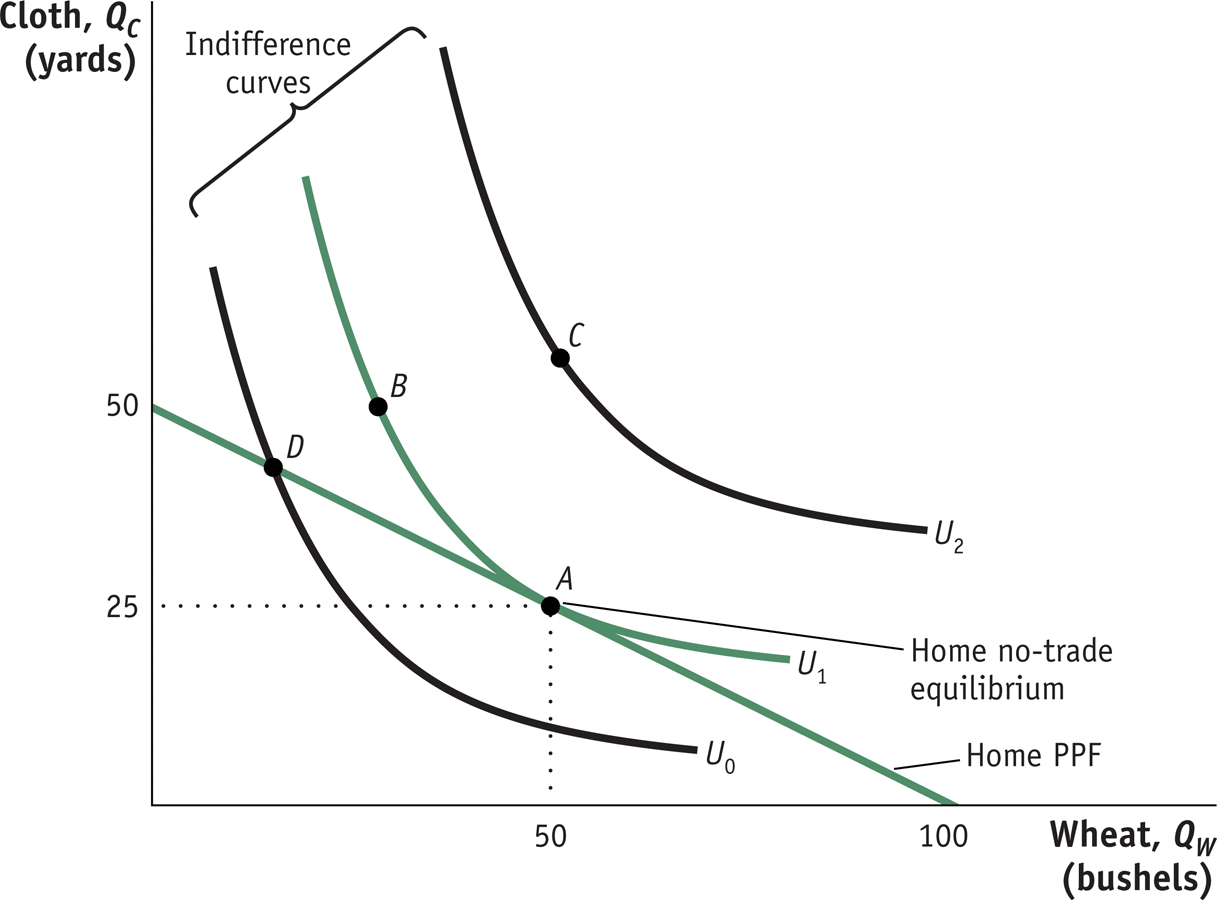
\includegraphics[height=3in,width=4.25in]{Feenstra_Essentials2e_fig_02_02.jpg}
\end{frame}

%%%%%%%%%%%%%%%%%%%%%%%%%%%%%%%%%%%%%%%%%%%%%%%%%%%%%%%%%%%%%%%%%%%%%%%%%%%%%%%%%%%%%%%%%%%%%%%%
%%%%%%%%%%%%%%%%%%%%%%%%%%%%%%%%%%%%%%%%%%%%%%%%%%%%%%%%%%%%%%%%%%%%%%%%%%%%%%%%%%%%%%%%%%%%%%%%

\begin{frame}[t]
\frametitle{Do at home\ldots}
\bigskip
\begin{itemize}
\item What is the Foreign country's opportunity cost of producing wheat?
\bigskip
\item What is the Foreign country's opportunity cost of producing cloth?
\bigskip
\item What is the autarky relative price of wheat?
\end{itemize}
\end{frame}

%%%%%%%%%%%%%%%%%%%%%%%%%%%%%%%%%%%%%%%%%%%%%%%%%%%%%%%%%%%%%%%%%%%%%%%%%%%%%%%%%%%%%%%%%%%%%%%%
%%%%%%%%%%%%%%%%%%%%%%%%%%%%%%%%%%%%%%%%%%%%%%%%%%%%%%%%%%%%%%%%%%%%%%%%%%%%%%%%%%%%%%%%%%%%%%%%


\begin{frame}[t]
\frametitle{Where we are going next\ldots}
\bigskip
\begin{itemize}
\item Pattern of trade.
\bigskip
\item Prices at which countries are willing to trade internationally.
\bigskip
\item Gains from trade.
\end{itemize}
\end{frame}




\end{document} 